\documentclass[10pt,a4paper]{article}

\usepackage[margin=1.7cm,top=1.4cm,bottom=1.4cm]{geometry}
\usepackage[T1]{fontenc}
\usepackage[utf8]{inputenc}
\usepackage{mathptmx}
\usepackage{amsmath,amssymb}
\usepackage{booktabs}
\usepackage{array}
\usepackage{enumitem}
\usepackage{xcolor}
\usepackage{fancyhdr}
\usepackage{titlesec}
\titlespacing*{\section}{0pt}{7pt}{3pt}
\titleformat*{\section}{\normalsize\bfseries\color{navy}}
\usepackage[colorlinks=true,linkcolor=black,urlcolor=blue!60!black]{hyperref}
\usepackage{graphicx}
\usepackage{listings}
\lstset{
  language=Python,
  basicstyle=\ttfamily\scriptsize,
  keywordstyle=\color{navy}\bfseries,
  commentstyle=\color{gray!80!black}\itshape,
  stringstyle=\color{green!40!black},
  numbers=left, numberstyle=\tiny\color{gray}, numbersep=6pt,
  breaklines=true, breakatwhitespace=true,
  showstringspaces=false, tabsize=4,
  frame=single, framerule=0.3pt, rulecolor=\color{gray!60},
  xleftmargin=2em, columns=fullflexible, keepspaces=true
}

% ---------- Report information (edit here) ----------
\newcommand{\myname}{Arnab Kumar Ghosh}
\newcommand{\reporttitle}{Progress Report}
\newcommand{\projecttitle}{Discrete State-Space Models and Expectation-Maximization for Cell-State Trajectories}
\newcommand{\supervisor}{Prashant Singh}
\newcommand{\period}{Weeks 3--4}
\newcommand{\reportdate}{\today}
% ----------------------------------------------------

\definecolor{navy}{RGB}{31,56,100}
\setlist{nosep, leftmargin=1.4em}
\setlength{\parskip}{2pt}
\AtBeginDocument{\setlength{\abovedisplayskip}{4pt}\setlength{\belowdisplayskip}{4pt}}
\setlength{\parindent}{0pt}

\pagestyle{fancy}
\fancyhf{}
\rhead{\small Progress report -- \period}
\cfoot{\small\thepage}
\renewcommand{\headrulewidth}{0.3pt}

\newcommand{\sub}[1]{\vspace{1pt}\textbf{\textcolor{gray!80!black}{#1}}\par}

\begin{document}

% ---------- Title block ----------
\begin{center}
  {\Large\bfseries\textcolor{navy}{\reporttitle}}\\[2pt]
  {\projecttitle}\\[3pt]
  {\small \myname\ \textperiodcentered\ Supervisor: \supervisor\ \textperiodcentered\ MSc Computer Science, Uppsala University \textperiodcentered\ \period\ \textperiodcentered\ \reportdate}
\end{center}
\vspace{-2pt}
\hrule
\vspace{4pt}

% ---------- 0. Overview ----------
\section*{Overview}
In weeks 3--4 I moved from the model definition to the algorithms. The open question from the last report (how to build the observation sequence) was discussed with the supervisor in the meeting on 22 September, but I still have questions about it (Section 7). Progress against the plan from the last report:

\begin{itemize}
  \item Forward and backward algorithms with per-step scaling (Rabiner Problem 1): \textbf{done}, on paper and in code.
  \item Posteriors $\gamma_t(i)$ and $\xi_t(i,j)$, i.e.\ the E-step: \textbf{done} in code.
  \item Baum--Welch re-estimation (Rabiner Problem 3) for discrete emissions: \textbf{done} in code, with checks.
  \item Sequence definition: discussed with the supervisor; still open, see Section 7.
  \item Bilmes (1998) and the Gaussian-emission M-step: \textbf{not yet}.
  \item Data received from the biology group, with a read-me describing the dataset.
  \item Read the previous student's internship report and identified why its results went wrong (Section 6).
\end{itemize}

The toy implementation is a small NumPy script: $N = 3$ states, $M = 4$ discrete symbols, known parameters $\lambda = (A, B, \pi)$, a sampler to generate sequences, and one function per algorithm. The rest of this report summarises what I understand so far and how each part connects to the project.

% ---------- 1 ----------
\section{The forward algorithm (Rabiner, Problem 1)}

\sub{What I learned}
The hidden state at time $t$ is $s_t$, the observation sequence is $O = o_1 \cdots o_T$, and the model is $\lambda = (A, B, \pi)$ with
\begin{align*}
A[i,j] &= P(s_{t+1} = j \mid s_t = i), && \text{transition: from state $i$ to state $j$,} \\
B[j,k] &= P(o_t = k \mid s_t = j), && \text{emission: state $j$ produces symbol $k$,} \\
\pi_i &= P(s_1 = i). && \text{start in state $i$.}
\end{align*}
In the code these are the arrays \texttt{A}, \texttt{B} and \texttt{pi}.

The forward variable is the probability of seeing the first $t$ observations and ending in state $i$:
\[
\alpha_t(i) = P(o_1 \cdots o_t,\; s_t = i \mid \lambda).
\]
It is filled in one time step at a time, and the last row gives the likelihood of the whole sequence:
\begin{align*}
\alpha_1(i) &= \pi_i\, B[i,o_1], \\
\alpha_t(j) &= \Big[ \sum_{i=1}^{N} \alpha_{t-1}(i)\, A[i,j] \Big]\, B[j,o_t], \\
P(O \mid \lambda) &= \sum_{i=1}^{N} \alpha_T(i).
\end{align*}
The sum inside the bracket is ``all the ways to arrive in state $j$'', and the factor $B[j,o_t]$ is ``and then see the new observation''. This replaces the sum over all $N^T$ state paths with a table of $N \times T$ numbers.

\sub{In the project}
$P(O \mid \lambda)$ is the likelihood of the data under the current parameters. It is the quantity that must never decrease during Baum--Welch, so the forward algorithm is also the tool for checking that training is working.

% ---------- 2 ----------
\section{The backward algorithm and the posteriors (E-step)}

\sub{What I learned}
The backward variable is the probability of the rest of the sequence, given that the state at time $t$ is $i$:
\[
\beta_t(i) = P(o_{t+1} \cdots o_T \mid s_t = i, \lambda).
\]
It is filled in from the end:
\begin{align*}
\beta_T(i) &= 1, \\
\beta_t(i) &= \sum_{j=1}^{N} A[i,j]\, B[j,o_{t+1}]\, \beta_{t+1}(j).
\end{align*}
Together, $\alpha$ and $\beta$ give the two posteriors needed by EM. $\gamma_t(i)$ is the probability of being in state $i$ at time $t$, and $\xi_t(i,j)$ the probability of being in state $i$ at time $t$ and in state $j$ at time $t+1$, both given the whole sequence:
\begin{align*}
\gamma_t(i) &= \frac{\alpha_t(i)\, \beta_t(i)}{P(O \mid \lambda)}, \\
\xi_t(i,j) &= \frac{\alpha_t(i)\, A[i,j]\, B[j,o_{t+1}]\, \beta_{t+1}(j)}{P(O \mid \lambda)} .
\end{align*}
$\alpha$ carries the evidence from the past, $\beta$ the evidence from the future, and $\gamma$ combines both. In the code, $\gamma$ rows sum to 1, every $\xi_t$ slice sums to 1, and $\sum_j \xi_t(i,j) = \gamma_t(i)$; these are asserted after every run.

\sub{In the project}
$\gamma_t(i)$ is, for each cell, the probability of being a Macrophage, Transitional or Mural-like cell. On the toy data, $\arg\max_i \gamma_t(i)$ recovers the true state at most time steps, which is how cells could be labelled later.

% ---------- 3 ----------
\section{Scaling (the numerical issue from the last report)}

\sub{What I learned}
Every $\alpha_t(i)$ is a product of $t$ probabilities, so it underflows to zero for long sequences. The standard fix is to divide each row of $\alpha$ by its sum and remember that sum as the scale factor:
\begin{align*}
c_t &= \sum_{i=1}^{N} \alpha_t(i), \\
\hat{\alpha}_t(i) &= \frac{\alpha_t(i)}{c_t}, \\
\log P(O \mid \lambda) &= \sum_{t=1}^{T} \log c_t .
\end{align*}
$\beta$ is scaled with the same factors, but row $t$ is divided by $c_{t+1}$, because $\beta_t$ covers the future observations $o_{t+1} \cdots o_T$ while $\alpha_t$ already covers $o_1 \cdots o_t$. Then $\hat{\alpha}_t(i)\, \hat{\beta}_t(i)$ sums to 1 at every $t$ and $\gamma$ is simply $\hat{\alpha}\, \hat{\beta}$, so the posteriors are unchanged. In the code the forward and backward passes each compute the log-likelihood independently and the two values agree to machine precision, which is the check that the scaling is consistent.

\sub{In the project}
The implementation uses scaling from the start, as agreed with the supervisor, so the log-likelihood check is always well defined.

% ---------- 4 ----------
\section{Baum--Welch re-estimation (Rabiner, Problem 3)}

\sub{What I learned}
The M-step turns the posteriors into new parameters. Every update is a normalised expected count: expected number of transitions from $i$ to $j$ over expected number of visits to $i$, and expected number of visits to $j$ that emit symbol $k$ over expected number of visits to $j$:
\begin{align*}
\bar{\pi}_i &= \gamma_1(i), \\
\bar{A}[i,j] &= \frac{\sum_{t=1}^{T-1} \xi_t(i,j)}{\sum_{t=1}^{T-1} \gamma_t(i)}, \\
\bar{B}[j,k] &= \frac{\sum_{t:\, o_t = k} \gamma_t(j)}{\sum_{t=1}^{T} \gamma_t(j)} .
\end{align*}
Baum--Welch repeats E-step and M-step until the log-likelihood stops increasing. I tested it on a sequence of 2000 toy observations sampled from the true $\lambda$, starting from five different random parameter sets (Figure~\ref{fig:baum_welch}). Panel (a) shows the log-likelihood after every iteration. Every curve rises monotonically: it never goes down, which the code asserts. The dashed line is the log-likelihood under the true parameters ($-2698.1$). Four of the five starts end slightly \emph{above} this line (about $-2688$). This is not an error. The true parameters describe the generating process, while Baum--Welch tunes the parameters to this one finite sample, including its random noise, so it can fit the sample a little better. The fifth start (start 2) ends lower, at $-2697.5$: it climbed a different hill and stopped at a local optimum.

Panel (b) shows why the fitted $B$ does not look like the true one even for a good start. The middle matrix is what Baum--Welch returns for start 4: the rows are the true rows in a different order. This is label switching. The state names S1, S2, S3 are arbitrary, and renaming the states gives exactly the same likelihood, so Baum--Welch cannot know which fitted state should be called S1. Once the rows are re-ordered to match (right matrix) the fitted $B$ is close to the true $B$. So two things are needed to recover the generating parameters: several random restarts, keeping the best log-likelihood, to avoid local optima such as start 2; and matching the state labels before comparing with the truth.

\begin{figure}[h]
  \centering
  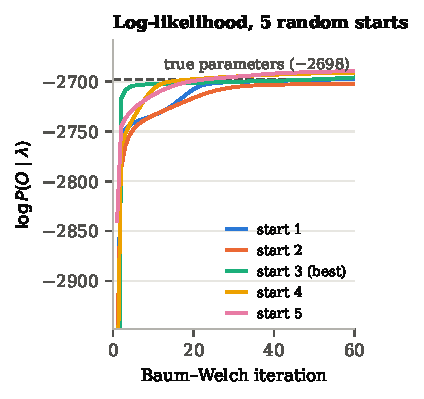
\includegraphics[width=\textwidth]{figures/baum_welch.pdf}
  \caption{Baum--Welch on 2000 toy observations. (a) Log-likelihood per iteration for five random starts; the dashed line is the value under the true parameters. Every curve rises monotonically, four starts end slightly above the true value and one (start 2) stops at a lower local optimum. (b) The emission matrix $B$: the true $B$, the fitted $B$ for start 4 as returned (rows in a different order: label switching), and the same matrix after re-ordering the rows to match the true states. Produced by \texttt{plot\_baum\_welch.py}, 200 iterations per start.}
  \label{fig:baum_welch}
\end{figure}

\sub{In the project}
This is the training loop the project needs. The $\bar{A}[i,j]$ and $\bar{\pi}_i$ updates carry over unchanged; only $\bar{B}[j,k]$ has to be replaced by the updates for the Gaussian mean $\mu_j$ and covariance $U_j$ from Bilmes. The local-optimum behaviour is a warning for the real data: several restarts and a comparison with the known labels will be necessary.

% ---------- 5 ----------
% Commented out for now: still have open questions about the population-level model.
\iffalse
\section{Sequence definition: resolved}

\sub{What was decided}
scRNA-seq measures each cell only once, so no single cell can be followed over time. The three ways of building a per-cell sequence were discussed and all rejected: ordering cells by time point only reflects the construction, random pairing of cells across time points invents transitions that were never observed, and a pseudotime-ordered HMM mostly relearns the pseudotime construction rather than the biology.

The chosen direction is a \textbf{population-level model}. Let $p_t$ be the row vector of state proportions on day $t$, so $p_t(j)$ is the fraction of cells in state $j$. Then
\[
p_{t+1}(j) = \sum_{i=1}^{N} p_t(i)\, A[i,j] ,
\]
with one step of $A$ per 7 days, matching the time points in the data. On day $t$ the cells are a mixture of the three state Gaussians with weights $p_t$, and the Gaussians are shared across all days:
\begin{align*}
P(O \mid \text{day } t) &= \sum_{j=1}^{N} p_t(j)\; B[j,O], \\
B[j,O] &= \mathcal{N}(O;\, \mu_j, U_j).
\end{align*}

\sub{In the project}
The meaning of $A$ changes slightly but stays the main result: $A[i,j]$ is now the fraction of the population moving from state $i$ to state $j$ per week. The model is still fitted by EM: the E-step gives per-cell state probabilities exactly like $\gamma$ above, the Gaussian means and covariances update in closed form, and $A$ needs a small numerical optimisation in the M-step because the proportions on different days are linked through the same matrix. Validation is by comparing the modelled state proportions $p_t$ with the observed proportions at each time point.

\fi

% ---------- 6 ----------
\section{The dataset}

\sub{What I learned}
The data arrived as \texttt{adata\_final.h5ad}, a combination of two single-cell sets (ss2 and ss3). ss2 covers day 21 and healthy tissue; ss3 covers days 7, 14, 21 (few cells) and healthy. So days 7 and 14 come only from ss3, while day 21 comes mostly from ss2: a difference between day 7/14 and day 21 can be partly protocol rather than biology. The read-me notes that the pseudotime looks the same on ss2 alone and on ss2+ss3, which suggests the batch effect is not dominant, but I will keep the batch label per cell. The three states of the model map onto labels that already exist in the data:

\begin{center}
\renewcommand{\arraystretch}{1.1}\small
\begin{tabular}{@{}>{\raggedright\arraybackslash}p{3.2cm} >{\raggedright\arraybackslash}p{5.6cm} >{\raggedright\arraybackslash}p{7.4cm}@{}}
\toprule
\textbf{Model state} & \textbf{Label in the data} & \textbf{Note} \\
\midrule
Macrophage & \texttt{cell\_type} = ``Macrophages'' & Starting population after injury \\
Transitional & \texttt{cluster} = 2 (PDGFRb$^{+}$ macrophages) & Almost absent at day 7 and 14, many at day 21; high unspliced-mRNA fraction, a sign of active reprogramming \\
Mural-like & \texttt{cell\_type} = ``Mural cells'', \texttt{cluster} = 8 & Marker genes include \textit{Pdgfrb}, \textit{Acta2}, \textit{Myh11}, \textit{Notch3} \\
\bottomrule
\end{tabular}
\end{center}

\sub{In the project}
The existing labels will be used only as an external check of the fitted states, not as training input. The observation vector $O$ for each cell will be the expression of the 50 genes listed in the read-me: the top 25 marker genes of cluster 2 (PDGFRb$^{+}$ macrophages) and the top 25 of cluster 8 (mural cells). A Gaussian over all genes is not feasible, and these 50 were agreed with the supervisor as the starting point.

% ---------- 7 ----------
\section{The previous student's report}

\sub{What I learned}
I read the internship report of the previous student. He built the same three algorithms (forward--backward, Viterbi, Baum--Welch) in Python. To get observations, he ran $k$-means on three marker genes and gave each cell one of three labels. Then he put all cells in one long list, sorted by day, and used that list as the observation sequence. He describes two problems he could not solve:
\begin{enumerate}
  \item With a random start, Baum--Welch ended in a poor local maximum and the result made no biological sense. So he set $\pi$, $A$ and $B$ by hand to match the paper. I saw the same thing on my toy data (Section 4). The problem with his fix is that if you start from the answer you expect, you mostly get that answer back. Also, any entry set to 0 in $A$ stays 0 forever.
  \item His result said 100\,\% of cells are intermediate on day 7 and 100\,\% are mural on day 21. The paper says about 10\,\% and 20\,\%. The reason is how the sequence was built. Each cell in the list counts as one time step, so there are thousands of steps but the state only changes a few times (at the day boundaries). Baum--Welch therefore learns that changing state is almost impossible ($A$ has 0.993, 0.999 and 1.0 on the diagonal). Viterbi then gives the same state to every cell in a day block. So the proportions can only be 0\,\% or 100\,\%. This comes from the construction, not from the biology.
\end{enumerate}

\sub{In the project}
This supports the direction agreed with the supervisor. In the population-level model, one step of $A$ is one week, not one cell. Cells within a day are a mixture, so proportions can be any value. Emissions are Gaussians on real expression values, not $k$-means labels. Per-cell states come from $\gamma$, not from one Viterbi path. I will also use several random restarts and start from the data, not from the expected answer.

% ---------- 8 ----------
\section{What is still unclear to me}

\begin{itemize}
  \item Sequence definition. scRNA-seq measures each cell only once, so no single cell can be followed over time, and I do not yet see what the observation sequence $o_1 \cdots o_T$ should be. Ordering all cells by day makes every cell a time step, which is the construction that went wrong in the previous student's report (Section 6). The supervisor suggested a population-level view, where one step of $A$ is one week and the cells on a day are a mixture of the states, but I am not yet sure how this is written as an HMM likelihood and how it is fitted. This is my main question for the next meeting.
  \item The Gaussian-emission M-step (Bilmes): how the $\bar{B}[j,k]$ update above becomes updates for $\mu_j$ and $U_j$, and how to keep $U_j$ well conditioned when a state has few cells.
  \item How to deal with local optima in practice: how many restarts, and how to pick between fits that differ only by label switching.
  \item Which matrix in \texttt{adata\_final.h5ad} to use for the 50 genes. The scaled \texttt{.X} matrix contains negative values, while \texttt{.raw.X} is log-normalised and non-negative; which one is suitable for Gaussian emissions, and does it matter that \textit{Pdgfrb} is missing from \texttt{.X}.
\end{itemize}

% ---------- 9 ----------
\section{Plan for the next two weeks}

\begin{itemize}
  \item Read Bilmes (1998): Gaussian mixture example first, then the HMM case. Replace the discrete $B[j,k]$ in the toy code by 1D and then 2D Gaussians and check that the known means and variances are recovered.
  \item Add several random restarts to the toy Baum--Welch and keep the best log-likelihood; check parameter recovery after matching the state labels.
  \item Open \texttt{adata\_final.h5ad}, check the normalisation, and compute the state proportions per time point.
  \item Write down the population-level likelihood and its E-step and M-step with the supervisor before fitting anything to the real data.
  \item Set up the validation agreed in the meeting: simulate cells from a fitted model and compare, gene by gene, the simulated and the real distribution of expression values.
\end{itemize}

\clearpage
\appendix
\section{Code: \texttt{hmm.py}}
The toy implementation discussed in Sections 1--4: scaled forward and backward passes, the posteriors $\gamma$ and $\xi$, Baum--Welch re-estimation, and the consistency checks. The file is included verbatim from \texttt{project-code/hmm.py}.

\lstinputlisting{../project-code/hmm.py}

\end{document}
